\documentclass[a4paper,12pt]{article}
\usepackage[utf8]{inputenc}
\usepackage[MeX]{polski}
\usepackage{fixltx2e}            %textsubscript
\usepackage{graphicx}
%%%%%%%%%%%%%%%%%%%%%%%%%%%%%%%%%%%%%%%%%%%%%%%%%%%%%%%%%%%%%STRONA TYTULOWA%%%%%%%%%%%%%%%%%%%%%%%%%%%%%%%%%%%%%%%%%%%%%%%%%%%%%%%%%%%%%%%%%%%%%%%%
\title{\Huge \textbf{Politechnika Wrocławska\\[0.3in]} 
  \huge Katedra Teorii Pola, Układów elektronicznych i Optoelektronicznych \\[0.2in]
  \LARGE Zespół Układów Elektronicznych
}
\date{}
\author{}

\begin{document}
\maketitle
\begin{table}[h]
  \large
  \centering
  \begin{tabular}{|ll|l|}
    \hline
    \multicolumn{1}{|l|}{Data: 7.04.2015r}                & \multicolumn{2}{l|}{Dzień: Wtorek}                                         \\ \hline
    \multicolumn{1}{|l|}{Grupa: VII}                      & \multicolumn{2}{l|}{Godzina: 12:15-15:00}                                  \\ \hline
    \multicolumn{3}{|l|}{\textit{\begin{tabular}[c]{@{}l@{}}\textbf{Temat ćwiczenia:} \\ Przerzutnik astabilny ``555''\end{tabular}}} \\ \hline
    \textbf{Dane projektowe:}                             & \multicolumn{2}{l|}{}                                                      \\
    T=0.50 \mu s                                          & \multicolumn{2}{l|}{}                                                      \\
    C=4.7 nF                                               & \multicolumn{2}{l|}{}                                                      \\
    R\textsubscript{a}=10k \Omega                         & \multicolumn{2}{l|}{}                                                      \\ \hline
    \multicolumn{1}{|l|}{\textbf{l.p}}                    & \textbf{Nazwisko i imię}                 & \textbf{Oceny}                  \\ \hline
    \multicolumn{1}{|l|}{1}                               & Arkadiusz Ziółkowski                     &                                 \\ \hline
    \multicolumn{1}{|l|}{2}                               & Jakub Koban                              &                                 \\ \hline
  \end{tabular}
\end{table}


%%%%%%%%%%%%%%%%%%%%%%%%%%%%%%%%%%%%%%%%%%%%%%%%%%%%%%%%%%%%%%%%%%%%%%%%%%%%%%%%%%%%%%%%%%%%%%%%%%%%%%%%%%%%%%%%%%%%%%%%%%%%%%%%%%%%%%%%%%%%%%%%%%%%
%%%%%%%%%%%%%%%%%%%%%%%%%%%%%%%%%%%%%%%%%%%%%%%%%%%%%%%%%%%%%%%%%%%ZADANIE PROJEKTOWE%%%%%%%%%%%%%%%%%%%%%%%%%%%%%%%%%%%%%%%%%%%%%%%%%%%%%%%%%%%%%%%
%%%%%%%%%%%%%%%%%%%%%%%%%%%%%%%%%%%%%%%%%%%%%%%%%%%%%%%%%%%%%%%%%%%%%%%%%%%%%%%%%%%%%%%%%%%%%%%%%%%%%%%%%%%%%%%%%%%%%%%%%%%%%%%%%%%%%%%%%%%%%%%%%%%%
\pagebreak
\section{Zadanie projektowe}
Zaprojektować przerzutnik monostabilny w oparciu o uład scalony ``555'' dla T=50 \mu s
%%%%%%%%%%%%%%%%%%%%%%%%%%%%%%%%%%%%%%%%%%%%%%%%%%%%%%%%%%%%%%%%%%%%%%%%%%%%%%%%%%%%%%%%%%%%%%%%%%%%%%%%%%%%%%%%%%%%%%%%%%%%%%%%%%%%%%%%%%%%%%%%%%%%
%%%%%%%%%%%%%%%%%%%%%%%%%%%%%%%%%%%%%%%%%%%%%%%%%%%%%%%%%%%%%%%%%%%CZĘŚĆ PROJEKTOWA%%%%%%%%%%%%%%%%%%%%%%%%%%%%%%%%%%%%%%%%%%%%%%%%%%%%%%%%%%%%%%%%%
%%%%%%%%%%%%%%%%%%%%%%%%%%%%%%%%%%%%%%%%%%%%%%%%%%%%%%%%%%%%%%%%%%%%%%%%%%%%%%%%%%%%%%%%%%%%%%%%%%%%%%%%%%%%%%%%%%%%%%%%%%%%%%%%%%%%%%%%%%%%%%%%%%%%
\subsection{Obliczenia projektowe}
\begin{equation} 
  \resizebox{0.9\hsize}{!}
  $ T=R_A\cdot C\cdot ln\left(\frac{V_{CC}}{V_{CC}-\frac{2}{3}V_{CC}}\right)\approx 1.1\cdot R_A\cdot C=1.1\cdot10 k\Omega\cdot 4.7nF  = 51\mu s $
\end{equation}
%%%%%%%%%%%%%%%%%%%%%%%%%%%%%%%%%%%%%%%%%%%%%%%%%%%%%%%%%%%%%%%%%%%%%%%%%%%%%%%%%%%%%%%%%%%%%%%%%%%%%%%%%%%%%%%%%%%%%%%%%%%%%%%%%%%%%%%%%%%%%%%%%%%%
\subsection {Schemat projektowy}   
\begin{figure}[h]
  \center
  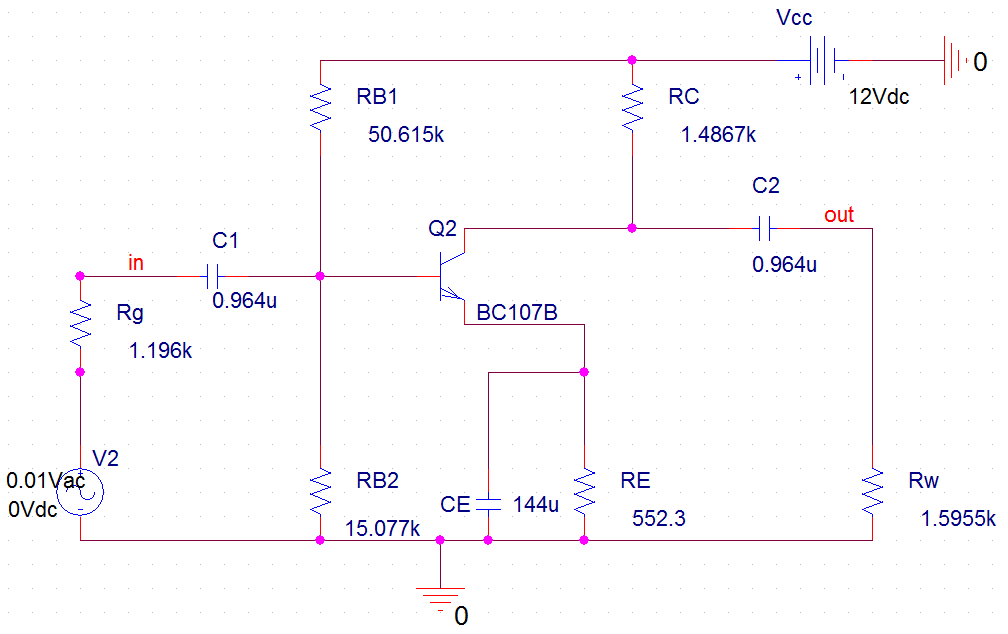
\includegraphics[width=1\textwidth]{schemat}
  \caption{Schemat projektowanego układu}
\end{figure}
\pagebreak
%%%%%%%%%%%%%%%%%%%%%%%%%%%%%%%%%%%%%%%%%%%%%%%%%%%%%%%%%%%%%%%%%%%%%%%%%%%%%%%%%%%%%%%%%%%%%%%%%%%%%%%%%%%%%%%%%%%%%%%%%%%%%%%%%%%%%%%%%%%%%%%%%%%%
%%%%%%%%%%%%%%%%%%%%%%%%%%%%%%%%%%%%%%%%%%%%%%%%%%%%%%%%%%%%%%%%%%%CZĘŚĆ LABORATORYJNA%%%%%%%%%%%%%%%%%%%%%%%%%%%%%%%%%%%%%%%%%%%%%%%%%%%%%%%%%%%%%%
%%%%%%%%%%%%%%%%%%%%%%%%%%%%%%%%%%%%%%%%%%%%%%%%%%%%%%%%%%%%%%%%%%%%%%%%%%%%%%%%%%%%%%%%%%%%%%%%%%%%%%%%%%%%%%%%%%%%%%%%%%%%%%%%%%%%%%%%%%%%%%%%%%%%
\section{Część laboratoryjna}
\subsection{Czas trwania impulsu jako funkcja napięcia wyjściowego}
%\begin{table}[h]
%\centering
%\begin{tabular}{|c|c|c|}
%\hline
%\textbf{T {[}$\mu$s{]} } & \textbf{U\textsubscript{wy}} & \textbf{Odchylenie [\%]} \\ \hline
%52.31              & 2.61                 & 2.41                       \\ \hline
%51.62              & 3.03                 & 1.06                       \\ \hline
%51.26              & 3.50                 & 0.35                       \\ \hline
%51.14              & 3.99                 & 0.12                       \\ \hline
%51.10              & 4.50                 & 0.04                       \\ \hline
%51.08              & 5.02                 & 0.00                       \\ \hline
%51.07              & 5.50                 & -0.02                      \\ \hline
%51.06              & 5.99                 & -0.04                      \\ \hline
%51.06              & 6.54                 & -0.04                      \\ \hline
%51.07              & 7.02                 & -0.02                      \\ \hline
%51.07              & 7.57                 & -0.02                      \\ \hline
%51.08              & 7.99                 & 0.00                       \\ \hline
%51.09              & 8.49                 & 0.02                       \\ \hline
%51.11              & 9.07                 & 0.06                       \\ \hline
%51.12              & 9.57                 & 0.08                       \\ \hline
%51.14              & 10.01                & 0.12                       \\ \hline
%51.16              & 10.53                & 0.16                       \\ \hline
%51.17              & 11.09                & 0.18                       \\ \hline
%51.19              & 11.49                & 0.22                       \\ \hline
%51.20              & 12.08                & 0.23                       \\ \hline
%51.21              & 12.50                & 0.25                       \\ \hline
%51.22              & 13.06                & 0.27                       \\ \hline
%51.23              & 13.52                & 0.29                       \\ \hline
%51.23              & 14.07                & 0.29                       \\ \hline
%51.23              & 14.52                & 0.29                       \\ \hline
%51.24              & 14.92                & 0.00                       \\ \hline
%\end{tabular}
%\end{table}
%%%%%%%%%%%%%%%%%%%%%%%%%%%%%%%%%%%%%%%%%%%%%%%%%%%%%%%%%%%%%%%%%%%%%%%%%%%%%%%%%%%%%%%%%%%%%%%%%%%%%%%%%%%%%%%%%%%%%%%%%%%%%%%%%%%%%%%%%%%%%%%%%%%%
\begin{figure}[h]
  \center 
  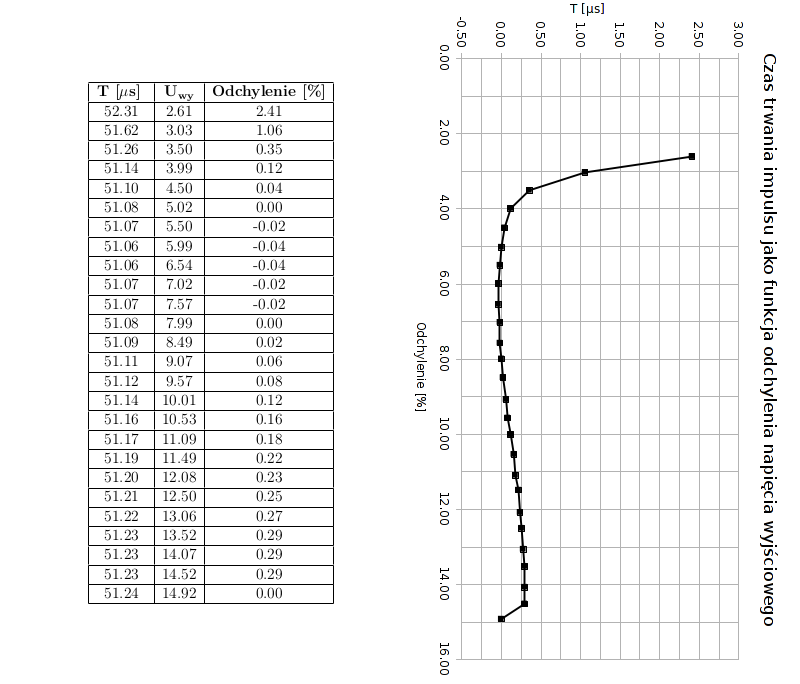
\includegraphics[width=0.9\textwidth]{tab}
  \caption{T=f(U\textsubscript{wy})}
\end{figure}
Na podstawie rys. 1 możemy wnioskować, iż czas trwania impulsu utrzymuje się na stałym poziomie ( odchylenie od wartości nominalnej wynosi maksymalnie 0.29\% ). Początek wykresu charakteryzuje się dużym odchyleniem, z uwagi na to, że przy tak małych napięciach układ nie zaczął jeszcze poprawnie pracować.
\pagebreak
%%%%%%%%%%%%%%%%%%%%%%%%%%%%%%%%%%%%%%%%%%%%%%%%%%%%%%%%%%%%%%%%%%%%%%%%%%%%%%%%%%%%%%%%%%%%%%%%%%%%%%%%%%%%%%%%%%%%%%%%%%%%%%%%%%%%%%%%%%%%%%%%%%%%
\subsection{Czas trwania impulsu jako funkcja napięcia modulacyjnego}
%\begin{table}[h]
%\left 
%\begin{tabular}{|c|c|}
%\hline
%\textbf{T {[}$\mu$s{]}]} & \textbf{U\textsubscript{mod} [V]} \\ \hline
%17.51     & 0.97      \\ \hline
%18.14     & 1.48      \\ \hline
%20.92     & 1.76      \\ \hline
%24.80     & 2.05      \\ \hline
%27.46     & 2.22      \\ \hline
%32.37     & 2.52      \\ \hline
%36.09     & 2.72      \\ \hline
%42.66     & 2.99      \\ \hline
%46.86     & 3.21      \\ \hline
%54.60     & 3.50      \\ \hline
%60.99     & 3.70      \\ \hline
%71.96     & 4.00      \\ \hline
%82.09     & 4.21      \\ \hline
%92.35     & 4.56      \\ \hline
%99.19     & 4.70      \\ \hline
%121.30    & 4.98      \\ \hline
%\end{tabular}
%\end{table}
%%%%%%%%%%%%%%%%%%%%%%%%%%%%%%%%%%%%%%%%%%%%%%%%%%%%%%%%%%%%%%%%%%%%%%%%%%%%%%%%%%%%%%%%%%%%%%%%%%%%%%%%%%%%%%%%%%%%%%%%%%%%%%%%%%%%%%%%%%%%%%%%%%%%
\begin{figure}[h]
  \centering
  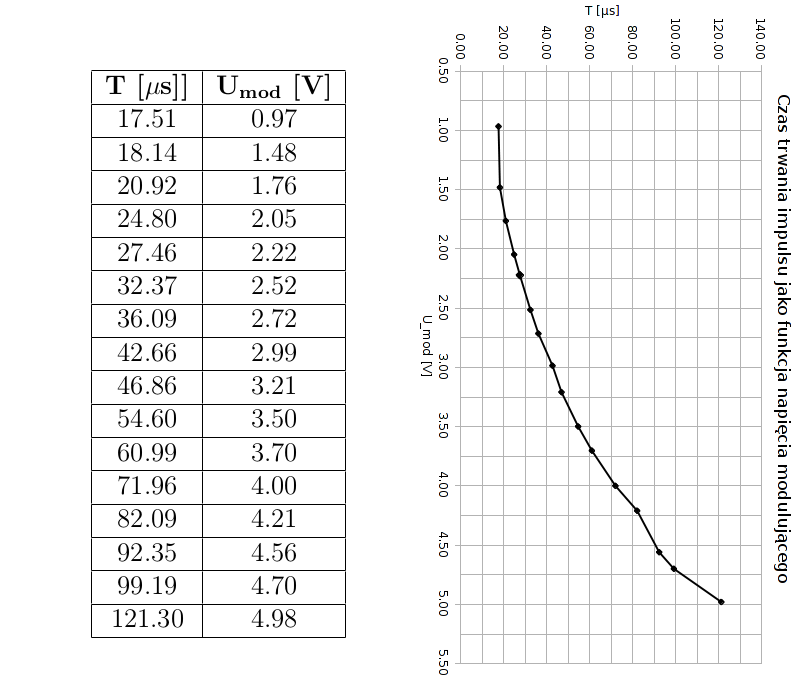
\includegraphics[width=0.9\textwidth]{tab2}
  \caption{T=f(U\textsubscript{wy})}
\end{figure}

Na podstawie rysunku nr.2 możemy wnioskować, iż wraz ze wzrostem napięcia modulującego długość impulsów rośnie.
\pagebreak
%%%%%%%%%%%%%%%%%%%%%%%%%%%%%%%%%%%%%%%%%%%%%%%%%%%%%%%%%%%%%%%%%%%%%%%%%%%%%%%%%%%%%%%%%%%%%%%%%%%%%%%%%%%%%%%%%%%%%%%%%%%%%%%%%%%%%%%%%%%%%%%%%%%%
\section {Wnioski}
\begin{enumerate}  
\item 
\item
\item 
\end{enumerate}


\end{document}
